\subsection{Сборка, тестирование и исследование зависимостей программы, осуществляющей работу с базой данных через псевдографический интерфейс}

\subsubsection{Сборка программы}

Для сборки программы был подготовлен файл \texttt{CMakeLists.txt}, который задаёт проект на языке C, стандарт C99 и настраивает поиск необходимых библиотек --- \texttt{ncursesw} (через \texttt{PkgConfig}) и \texttt{zlib}. После их нахождения добавляется исполняемый файл \texttt{app}, которому передаются пути к заголовочным файлам и библиотеки для линковки.

Редактирование данного файла производилось в редакторе \texttt{nano}, ниже приведён псевдокод:

\begin{lstlisting}[language=C, caption=Файл CMakeLists.txt]
установить минимально необходимую версию cmake 3.10
задать имя проекта "znak_db" и язык программирования C

установить стандарт языка C на C99

поиск с помощью pkg-config библиотеки ncursesw (обязательно)
если не найдена, будет ошибка сборки

поиск установленной в системе библиотеки zlib (обязательно)

создать исполняемый файл "app" из файлов:
    - main.c
    - app.c

указать каталоги заголовочных файлов для target "app",
чтобы компилятор знал, где искать заголовки ncursesw

связать исполняемый файл "app" с:
    - найденной библиотекой ncursesw
    - найденной библиотекой zlib
\end{lstlisting}

После этого был создан каталог \texttt{build}, в который были сгенерированы файлы сборочной системы командой \texttt{cmake ..}, и выполнена сама сборка проекта с помощью утилиты \texttt{make}. На выходе получен исполняемый файл \texttt{app}, который связывается с найденными библиотеками.

Ход выполнения этих команд и процесс сборки приведён на скриншоте \ref{fig:Screenshot_2025-07-01_at_01.12.42.png}.

\screenshot{Screenshot_2025-07-01_at_01.12.42.png}{Конфигурация и сборка проекта с использованием CMake и Make}

Таким образом, проект был успешно собран с подключением библиотек \texttt{ncursesw} для реализации псевдографического интерфейса и \texttt{zlib} для вычисления контрольных сумм. Исполняемый файл готов к тестированию и дальнейшему исследованию его зависимостей через команду \texttt{ldd}.

\subsubsection{Тестирование программы}

Программа была протестирована вручную: с помощью псевдографического интерфейса вводились новые записи, выполнялся просмотр заголовка и содержимого базы данных, поиск по знаку зодиака и году рождения, а также добавление новых записей. Результаты работы программы представлены на приведённых скриншотах, которые демонстрируют все основные этапы и корректное функционирование программы.

\screenshot{Screenshot_2025-07-01_at_01.43.35.png}{Запуск программы. Отсутствие базы данных и запрос на ввод количества записей.}
\screenshot{Screenshot_2025-07-01_at_01.44.06.png}{Ввод первой записи: фамилии, знака зодиака и года рождения.}
\screenshot{Screenshot_2025-07-01_at_01.44.12.png}{Главное меню программы с выбором действий.}
\screenshot{Screenshot_2025-07-01_at_01.44.15.png}{Просмотр заголовка базы данных с указанием количества записей и контрольной суммы.}
\screenshot{Screenshot_2025-07-01_at_01.44.20.png}{Просмотр всех записей в базе данных в табличном виде.}
\screenshot{Screenshot_2025-07-01_at_01.44.33.png}{Запрос параметров для поиска по знаку зодиака и году рождения.}
\screenshot{Screenshot_2025-07-01_at_01.44.35.png}{Результаты поиска записей по заданным критериям.}
\screenshot{Screenshot_2025-07-01_at_01.46.06.png}{Добавление новой записи в базу данных.}
\screenshot{Screenshot_2025-07-01_at_01.46.13.png}{Просмотр обновлённой базы данных с двумя записями.}
\screenshot{Screenshot_2025-07-01_at_01.46.31.png}{Просмотр обновлённого заголовка базы данных с увеличенным количеством записей и новой контрольной суммой.}
\screenshot{Screenshot_2025-07-01_at_01.47.33.png}{Удаление файла базы данных перед повторным тестированием.}
\screenshot{Screenshot_2025-07-01_at_01.47.45.png}{Запуск программы без базы данных и ввод некорректного количества записей (-1).}
\screenshot{Screenshot_2025-07-01_at_01.47.48.png}{Сообщение о недопустимом количестве записей и предложение повторить ввод.}
\screenshot{Screenshot_2025-07-01_at_01.49.15.png}{Повторный запуск программы с вводом 20 записей.}
\screenshot{Screenshot_2025-07-01_at_01.50.06.png}{Ввод записи с некорректным годом рождения вне допустимого диапазона.}
\screenshot{Screenshot_2025-07-01_at_01.50.09.png}{Сообщение о недопустимом году рождения и повторный запрос.}
\screenshot{Screenshot_2025-07-01_at_01.50.58.png}{Повторный воод года рождения.}
\screenshot{Screenshot_2025-07-01_at_01.51.11.png}{Сообщение о пустом знаке зодиака и повторный запрос.}
\screenshot{Screenshot_2025-07-01_at_01.55.18.png}{Просмотр заголовка базы данных после ввода записей.}
\screenshot{Screenshot_2025-07-01_at_01.55.29.png}{Просмотр всех записей базы данных в табличном виде после ввода 20 элементов.}
\screenshot{Screenshot_2025-07-01_at_01.55.32.png}{Просмотр вротой страницы всех записей базы данных в табличном виде после ввода 20 элементов.}
\screenshot{Screenshot_2025-07-01_at_01.56.16.png}{Поиск среди множества записей по знаку зодиака \texttt{f} и году \texttt{2000}}
\screenshot{Screenshot_2025-07-01_at_01.56.59.png}{Поиск заведомо некорректными данными}
\screenshot{Screenshot_2025-07-01_at_01.57.51.png}{Добавление записи на имя \texttt{petrov v v}}
\screenshot{Screenshot_2025-07-01_at_01.58.00.png}{Просмотр содержимого второй страницы обновлённой базы данных.}
\screenshot{Screenshot_2025-07-01_at_01.58.10.png}{Просмотр заголовка новой базы данных после создания --- указано количество записей и контрольная сумма.}

\subsubsection{Просмотр бинарного файла базы данных в шестнадцатеричном виде}

Для проверки корректности структуры и содержимого бинарного файла базы данных была использована утилита \texttt{hexdump} с параметром \texttt{-C}, позволяющим вывести данные в шестнадцатеричном виде с расшифровкой в ASCII. На примере ниже видно, что файл начинается с сигнатуры \texttt{SEME} (в шестнадцатеричном виде \texttt{53 45 4D 45}), далее идут служебные поля заголовка (номер транзакции, количество записей, контрольная сумма CRC32), а затем записи о пользователях. Таким образом, структура файла полностью соответствует ожидаемому формату.

\screenshot{Screenshot_2025-07-01_at_03.18.28.png}{Шестнадцатеричный дамп бинарного файла базы данных, полученный с помощью \texttt{hexdump -C znak\_db}.}

\subsubsection{Исследование разделяемых библиотек и построение дерева зависимостей}

После выполнения задания и получения исполняемого файла программы были исследованы её зависимости от разделяемых библиотек с помощью команды \texttt{ldd}. На скриншоте приведён результат анализа исполняемого файла \texttt{app} и его библиотек.

\screenshot{Screenshot_2025-07-01_at_03.38.15.png}{Вывод команды \texttt{ldd} для программы и зависимых библиотек.}

На основании результатов команды \texttt{ldd} было построено рекурсивное дерево зависимостей программы (рис. \ref{fig:app-ldd-tree}).

\begin{figure}[H]
  \scalebox{.7}{
    \centering
    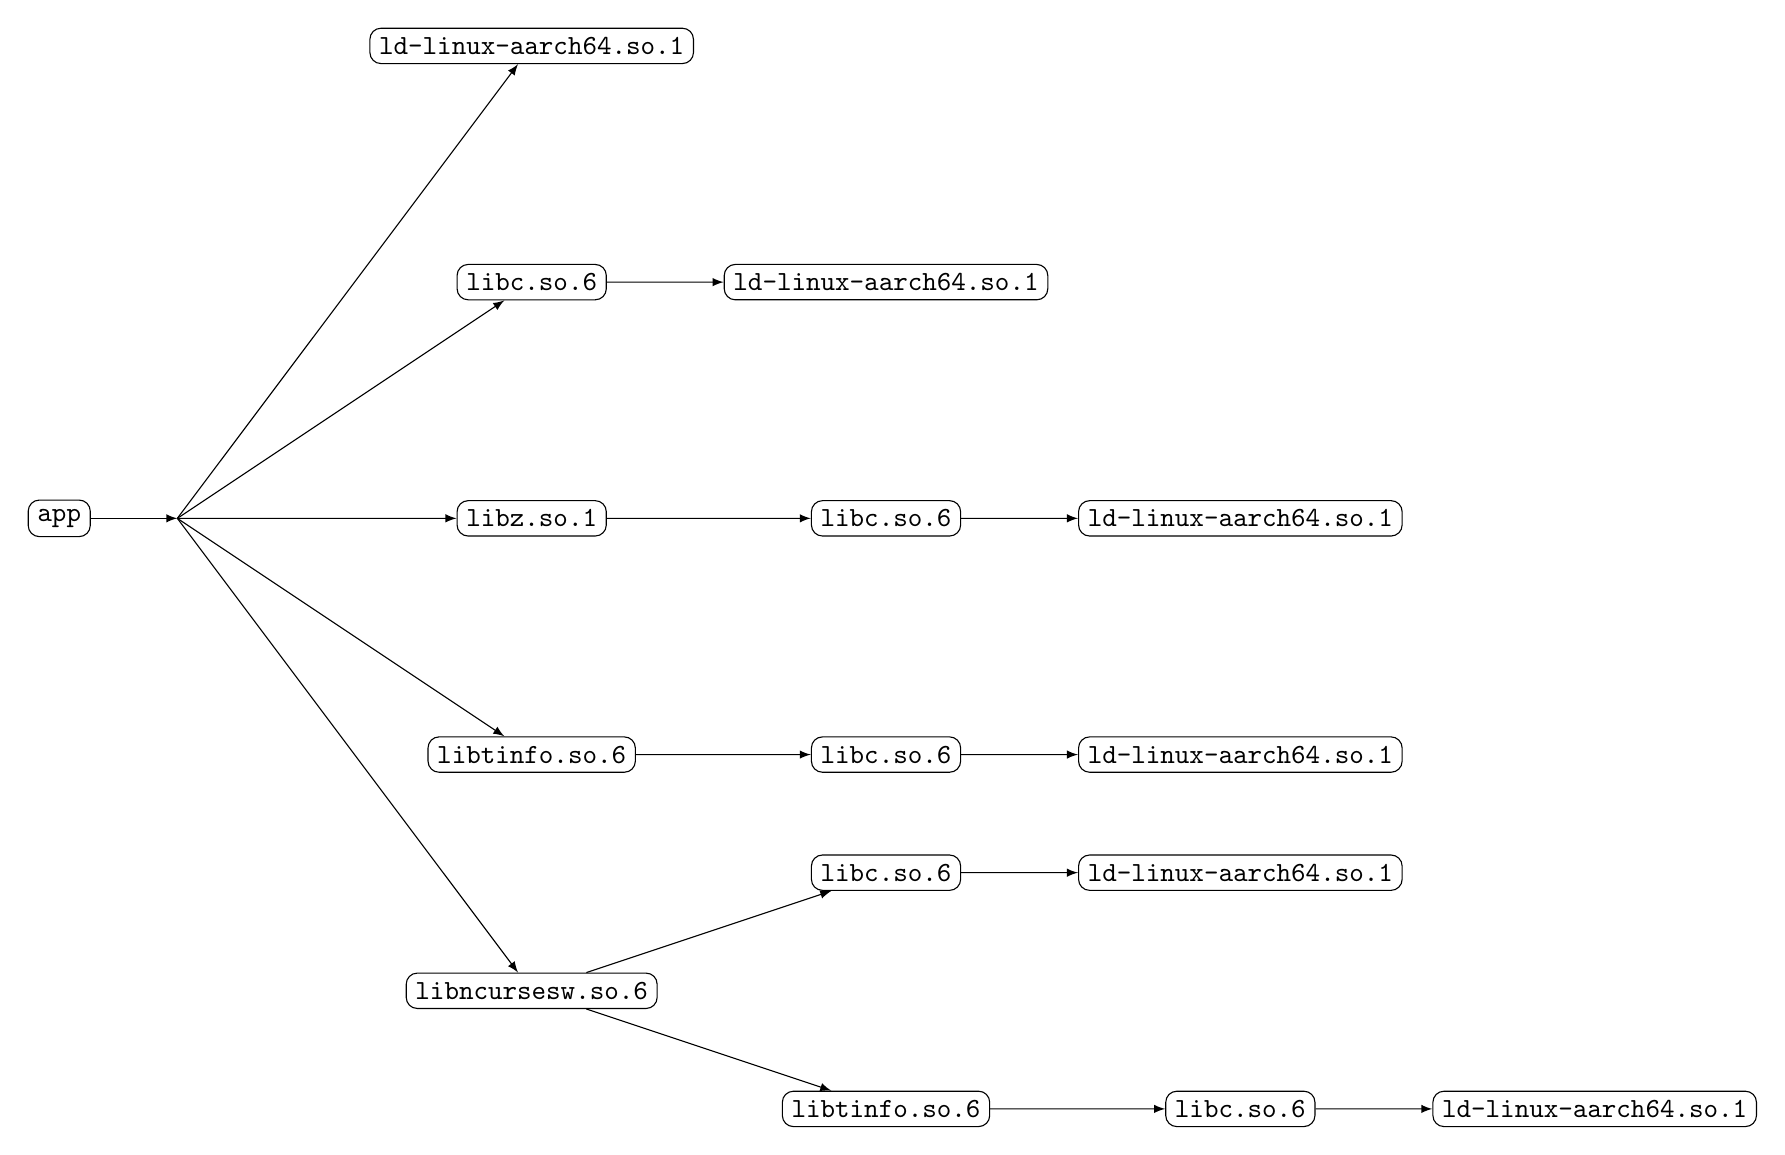
\begin{tikzpicture}[
    grow=down,
    level distance=4.5cm,
    sibling distance=3cm,
    edge from parent/.style={draw, -latex},
    every node/.style={draw=black, rounded corners, font=\ttfamily, align=left}
    ]
    
    \node {app}
    child[grow=right, xshift=-3cm] {
      child { node {libncursesw.so.6}
      child { node {libtinfo.so.6}
      child { node {libc.so.6}
      child { node {ld-linux-aarch64.so.1} }
      }
      }
      child { node {libc.so.6}
      child { node {ld-linux-aarch64.so.1} }
      }
      }
      child { node {libtinfo.so.6}
      child { node {libc.so.6}
      child { node {ld-linux-aarch64.so.1} }
      }
      }
      child { node {libz.so.1}
      child { node {libc.so.6}
      child { node {ld-linux-aarch64.so.1} }
      }
      }
      child { node {libc.so.6}
      child { node {ld-linux-aarch64.so.1} }
      }
      child { node {ld-linux-aarch64.so.1} }
    };
    
    \end{tikzpicture}
  }
\caption{Рекурсивное дерево зависимостей программы \texttt{app}, построенное с использованием \texttt{ldd}}
\label{fig:app-ldd-tree}
\end{figure}